\documentclass[10pt]{article}
\usepackage[margin=1in]{geometry}
\usepackage{amsmath}
\usepackage{graphicx}
\usepackage{authblk}

\title{Bridging measurements and simulations: A data assimilation approach to real time analysis}
\author{\underline{Ángel González Villatoro}, Mariachiara Gallia, David Rival}
\affil{Institut für Strömungsmechanik, Technische Universität Braunschweig, Germany }

\begin{document}
\maketitle

\begin{abstract}
Accurate simulation of wall-bounded turbulent flows remains challenging due to the high computational cost of resolving 
near-wall dynamics. Experimental techniques provide valuable data in this region, but are often limited by resolution. 
A promising strategy is to combine numerical simulations with wall-based measurements through data assimilation (DA) aiming 
to real-time .\\

In this work, we investigate which types of wall measurements are most effective for improving flow reconstruction 
while reducing computational cost. A sudden acceleration boundary-layer configuration, governed by the Navier–Stokes and 
energy equations, is used as the test case. High-resolution simulations provide the ground truth, from which 
synthetic wall observations (temperature, pressure, shear stress) are extracted and assimilated into a coarser simulation.\\

Four DA methods—nudging, Kalman Filter (KF), Ensemble Kalman Filter (EnKF), and 4D-Var—are benchmarked in terms of accuracy 
and efficiency. All methods achieve similar accuracy (RMSE (root mean square error) $\approx  0.13$), but with significant differences in cost. Nudging and KF 
provide the best balance, with nudging requiring less than 1 ms per update. EnKF enables multivariable assimilation at moderate 
cost, while 4D-Var achieves high accuracy but at the highest computational expense.
The results demonstrate the potential of lightweight DA approaches to integrate sparse wall-based experimental measurements 
into computational fluid dynamics workflows, bridging the gap between simulations and experiments.\\



\begin{figure}[h]
\centering
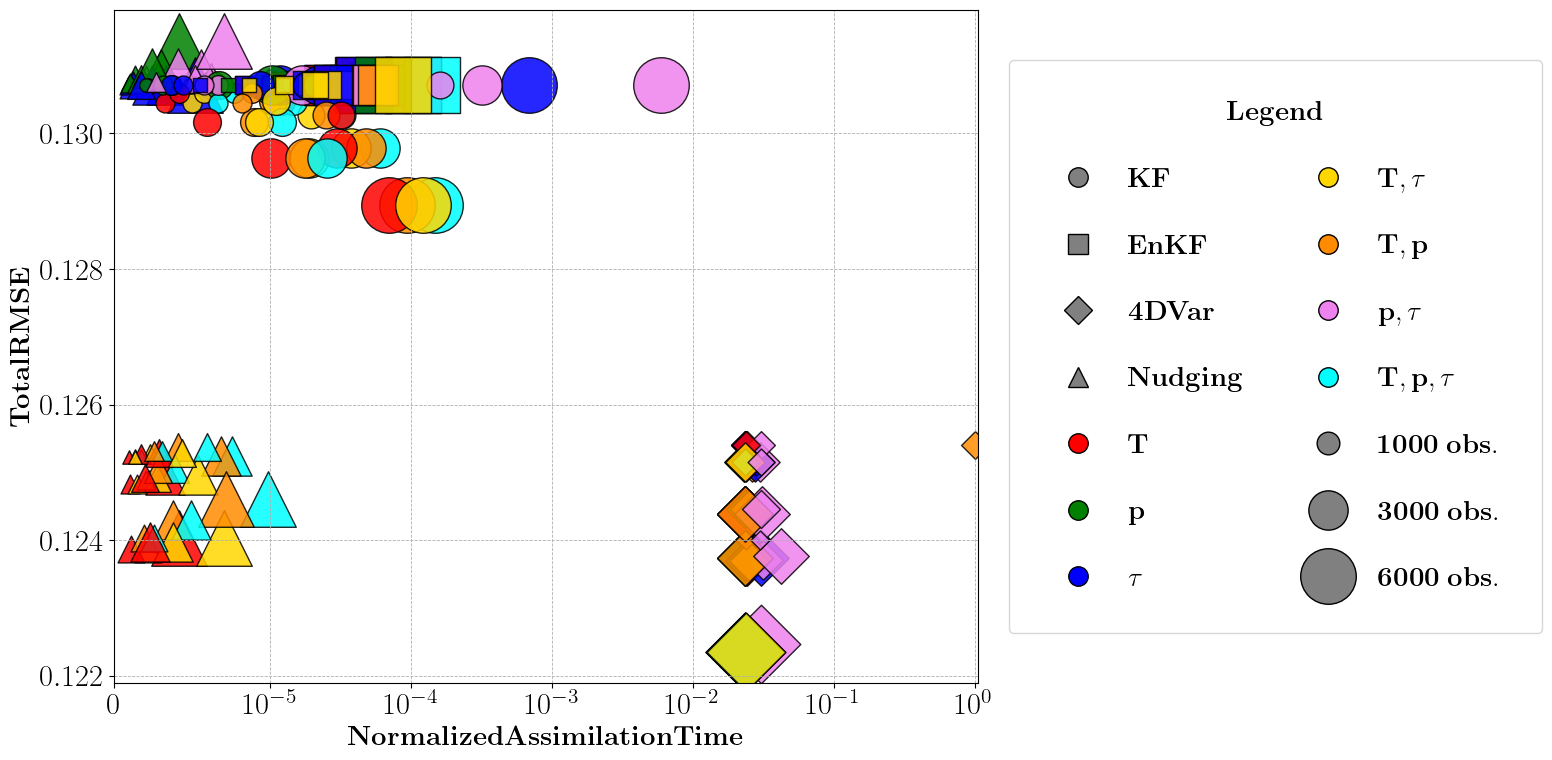
\includegraphics[width=0.75\textwidth]{total DA.png}
\caption{Accuracy (Total RMSE) versus normalized assimilation time for different DA methods. Marker shape = method, color = type of wall observation, size = number of observations.}
\end{figure}
\end{abstract}

\end{document}


